
\section{Introduction}

Advancements in quantum and particle physics are primarily driven by
experimental observations which can verify or refute previous hypotheses, or can
provide data from which new hypotheses can be drawn, with the overall goal
of helping us have a deeper understanding of the universe around us.
Particle colliders are a main source of observational data at the quantum scale,
and can create millions of collision events every second.  Design modifications
to these colliders mostly increase the luminosity of the collision in order to
increase the collision rate and produce more data.  This report however, focuses
on a design modification aimed at increasing the energy of the colliding beams.
Increasing the energy of particle colliders will give the ability to investigate
energy regions yet to be reached and allow the observation of interactions that
only happen at higher energies. These interactions may give insight into
questions pertaining to the unification of the fundamental forces.

% TODO
% Improvements to these colliders come in the form of increasing the luminosity
% of the beam.  beam energy come largely in the form of increasing the energy
% of the colliding particle beams.

Proton--proton beam energies at the Large Hadron Collider (LHC) have recently
reached energies of \SI{13}{\tera\electronvolt} \cite{CMS:2015bta}, whereas
lepton--lepton colliders have yet to reach the \si{\tera\electronvolt} energy
scale. The largest lepton--lepton collider, the Large Electron-Proton Collider (LEP),
was closed down to make way for the LHC in \num{2000} after having reached a
maximum energy of \SI{209}{\giga\electronvolt} \cite{Barate2003sz}.

% % TODO improve this explanation
% There are two main appeals of lepton--lepton colliders, both of which are due to 
% leptons being fundamental particles. The main 
% The precision of the centre-of-mass energy
% measurement is improved which will improve further calculation of 
% The cleanliness of lepton--lepton collisions is the main appeal of these
% colliders, since they are point-like fundamental particles with a controlled
% centre-of-mass energy.

One of the drawbacks to circular accelerators,
% for lighter particles especially,
is the loss of a particle's energy due to synchrotron radiation.  This is the
emittance of radiation from relativistic charged particles that are moving in a
uniform magnetic field. The energy loss is inversely proportional to the fourth
power of the rest mass of the particle \cite{sokolov1966synchrotron}, meaning
that electrons lose more energy than protons by a factor of about \num{e13}
which is.  During experiments performed at the LEP the radiated power when
running at \SI{100}{\giga\electronvolt} reached about \SI{18}{\mega\watt} which
needs to be resupplied to the beam.
% on-top of the power needed to accelerate the beam.

% TODO im not sure how much 18MW is.
% TODO should I talk about synchrotron radiation in the theory section?

% TODO talk more about the goals and location?
There are currently two RF linear lepton accelerator proposals, the Compact
Linear Collider (CLIC) and the International Linear Collider (ILC) which are
expected to reach collision energies of up to several \si{\tera\electronvolt}
and \SI{500}{\giga\electronvolt} respectively. Both collaborations have
recently joined efforts under the Linear Collider Collaboration.

Looking further into the future

continuing to increase the energy of colliding beams allows for an increasing
number of interactions to be observed.

% \begin{itemize}
% 	\item reasons why lepton collisions are cleaner than protons
% 	\item drawbacks of circular accelerator synchrotron radiation at LEP
% 		\cite{Brandt2000xk}
% 	\item ICL and CLIC proposed linear RF accelerators ten times larger
% 		than SLAC
% \end{itemize}

% however protons are
% not fundamental particles meaning the energy of each constituent particle is
% less than that of the beam. Leptons however, are fundamental point-like
% particles meaning their centre-of-mass energy can be determined to a higher
% precision and also the collision environment will be much cleaner.

% Looking at current accelerators, circular electron or positron accelerators are
% not possible at these energies unless the accelerator reaches the
% \SI{100}{\kilo\meter} scale as electrons at this energy approach the speed of
% light and since they are accelerating in a circle they will radiate large
% amounts of their energy.
% % \cite{sokolov1966synchrotron}
% An accelerator at the \SI{100}{\kilo\meter} scale is
% impractical due to geographical and financial limitations.  Similar problems
% also arise in linear colliders where current radio-frequency (RF) cavities in a
% linear collider will have to be tens of kilometres in length to reach the
% \si{\tera\electronvolt} scale, this is with current acceleration gradients of
% up to \SI{100}{\mega\volt\per\meter}.  This urges the development of a new
% methods for the acceleration of particles.

\section{Plasma Wakefield Acceleration}

Current radio-frequency (RF) accelerator technology is limited to an
electromagnetic gradient of about \SI{100}{\mega\electronvolt\per\meter} due to
material beakdown in the walls of the structure.  The ability of plasma to
sustain very large electromagnetic fields made it a good candidate for a medium
within which charged particles can be accelerated. In 1979, the concept of
laser plasma acceleration was shown in simulations to be of practial use in
accelerators and pulsers~\cite{Tajima:1979bn}. More recently, proof-of-concept
experiments implementing laser plasma acceleration have been shown to
accelerate electrons to the \si{\giga\electronvolt} scale in a
\si{\centi\metre}-scale plasma cell~\cite{Lu:2006nz,Leemans:2006dx}, showing
results that are consistent with simulations.

% The concept of accelerating particles in plasma was promising as plasma is able
% to sustain large electric fields.  The idea being that energy can be
% transferred to a group of charged particles by injecting them into the plasma
% wakefield that follows a high energy laser pulse or proton bunch, using the
% plasma as an energy transfer medium.  The witness bunch is then accelerated by
% the high electromagnetic gradient.

\subsection{Self-modulation instability}

The first challenge in the development of this accelerator was getting the
length of the proton driver bunch small enough so that resonance occurs with
the electrons in the plasma.  Typical proton bunches, i.e. those produced by
the CERN Super Proton Synchrotron (SPS), have lengths of \(\sim
\SI{10}{\centi\meter}\) which cannot directly create strong plasma waves at the
required wavelength in the \si{\milli\meter} scale as the Fourier component of
the proton beam at the plasma frequency is negligible.
Simulations~\cite{kumar2010self} on the compression of these bunches show that
reducing the longitudinal phase volume blows up the transverse phase volume.
An alternative method would be to split up the proton bunch into a number of
micro-bunches to be simultaneously decelerated.

An instability between the beam and the plasma arises from the mutual
amplification of the rippling of the beam radius and the plasma wave. This
instability tends to destroy the plasma wave as the amplification focuses and
defocuses selected slices of the beam.  This problem was solved by seeding the
self-modulated instability (SMI) with a short electron bunch
\cite{lotov2013natural}, a laser pulse \cite{siemon2013laser} or a sharp cut in
the bunch profile\cite{kumar2010self}. This will promote a single mode and
suppress other modes, including the strongest competing modes, the hosing modes
\cite{vieira2014hosing} and produce well-separated micro-bunches.

\subsection{Uniform-density plasma cell}

The plasma wavelength is \(\lambda_{pe} \approx \SI{1.26}{\milli\meter}\)
meaning that the \SI{10}{\centi\meter} proton bunch will have to be split into
\(\sim 100\) micro-bunches in order to be able to drive the wake.  Each
micro-bunch contributes to the wakefield, and only if the plasma density is
uniform will the contribution of each bunch be coherent. Incoherence will cause
the electron bunches to arrive at the wrong phase in the plasma oscillation. An
increase in the plasma density will shorten the plasma wavelength causing the
electron bunch to crest plasma wave it was riding and fall into the defocusing
phase of the plasma wave as shown in Fig \ref{fig:phases}(a). A decrease
in the plasma density will increase the plasma wavelength causing the plasma
wave to fall further behind the electron bunch meaning the electron bunch to
fall into the trough of the plasma wave resulting in a deceleration of the
electron beam \ref{fig:phases}(c). The electron beam must be in the
region of length \(\lambda_{pe}/4\) between the defocusing and decelerating
phases of the plasma wave.
% These effects are significantly larger for the electrons as protons have
% large longitudinal momentum.

\begin{figure}[tb]
	\centering
	\begin{subfigure}{\linewidth}
		\centering
		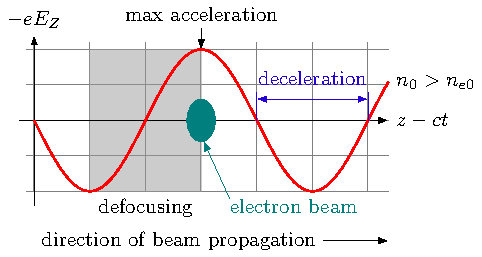
\includegraphics[width=0.9\linewidth]{figures/phases-a.pdf}
		\caption{asdkfjasdlfj sdk dfs f}
	\end{subfigure}
	\begin{subfigure}{\linewidth}
		\centering
		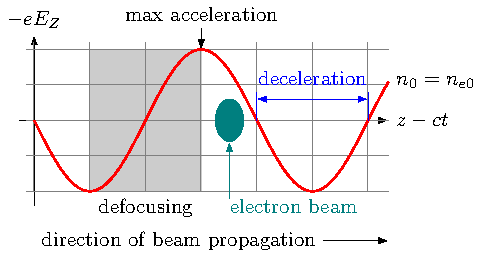
\includegraphics[width=0.9\linewidth]{figures/phases-b.pdf}
		\caption{asdkfjasdlfj sdk dfs f}
	\end{subfigure}
	\begin{subfigure}{\linewidth}
		\centering
		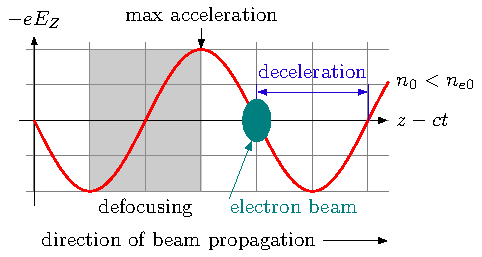
\includegraphics[width=0.9\linewidth]{figures/phases-c.pdf}
		\caption{asdkfjasdlfj sdk dfs f}
	\end{subfigure}
	\caption{
		Phasing of the electron bunch for increased density (a) correct density
		(b) and decreased density (c). \cite{wiedemann2007particle}
	}
	\label{fig:phases}
\end{figure}

This requirement of the plasma limits the plasma selection to being uniform
rubidium vapor, ionised by a co-propagating laser pulse \cite{oz2014novel,
oz2014bja}.  Rubidium was chosen due to it's low ionization potential and heavy
atomic mass.  A heavy element is required to minimize the movement of the
plasma's nuclei which causes adverse effects on the plasma's behaviour
\cite{vieira2012nj, vieira2014bqa}. The Rubiduim vapor is kept in thermodynamic
equilibrium at a constant temperature and volume.

\subsection{Injection of the witness beam}

Due to SMI, the shape of the drive beam changes in the plasma and for the first
four meters, the difference between the phase velocity of the wakefield and the
proton beam velocity is quite large and this will effect the electron beam in
the same manner as having a non uniform plasma, detailed above. To avoid this
problem it was suggested that the electrons could be injected into the plasma
after SMI had fully developed. The design of the injection method arrived at
passing the electron beam through a narrow vacuum tube separated from the
plasma by a thin foil. Then after \(\sim \SI{4}{\meter}\) the electrons will be
directed into the wakefield close close behind the proton driving beam.

